%---------------------------------------------------------------------
%
%                          Capítulo 4 - Descripción del problema
%
%---------------------------------------------------------------------

\chapter{Descripción del problema y soluciones propuestas}

\begin{quotation}\noindent\begin{small}\textbf{\spacedallcaps{RESUMEN}} \\
En este apartado se va a detallar el proceso que se ha seguido para llegar a la implementación final de la solución así como el desglose de la misma. En un primer momento, se definió de manera genérica el problema que se quería abordar. Tras esto, hubo varias reuniones con la usuaria final (que a su vez, es experta en esta materia) para definir tanto los requisitos funcionales como el diseño de la aplicación móvil y de la página web. Finalmente, podemos encontrar un resumen técnico de la implementación final basada en las conclusiones de las fases previamente mentadas.
\end{small}\end{quotation}


%-------------------------------------------------------------------
\section{Introducción}
\paragraph{}
A la hora de tratar clínicamente a un paciente con problemas de salud mental, existe el problema de que aquello que cuenta el paciente sobre su problema puede no corresponderse con la realidad. Así, mientras que si fuese un problema estrictamente fisiológico como puede ser un problema de tensión se podrían parametrizar las constantes vitales del paciente mediante aparatos médicos que sean independientes del sesgo del paciente, en el ámbito de la salud mental la causística es completamente distinta.

\paragraph{}
Un paciente puede acudir por voluntad propia o de terceros y tanto su versión como la interpretación de los hechos que le han llevado a la consulta pueden diferir severamente entre cada persona. Adicionalmente, tal y como se comentaba en la sección~\ref{subsubsec:intervencionPsico}, la ira se desarrolla en entornos muy específicos (y diferentes entre cada paciente), supone una distorsión intencionada de la realidad y, por la deseabilidad social del paciente, puede que niegue que tenga problemas de gestión de la ira a la hora de dirigirse al terapeuta.

\paragraph{}
Por todo ello, se propone una solución tecnológica que por un lado dé información adicional a la terapeuta para guiar la consulta para la gestión de la ira y, por otro, el paciente pueda tener en tiempo real información que le sea de utilidad para gestionar dicho episodio de ira. Concretamente, se propone un sistema tecnológico que mida las constantes fisiológicas del paciente, interprete si dicho patrón puede deberse a un episodio de ira y, en caso de que sea así, qué grado de la ira puede estar experimentando el paciente. Adicionalmente, estos episodios de ira se traducirán en pautas previamente confeccionadas por el terapeuta para cada grado de ira, con las que en el momento en el que se detecte la ira, el paciente tendrá una ayuda para poder gestionarla.

\paragraph{}
Para medir las constantes fisiológicas se utilizará una pulsera inteligente frente a otras alternativas como los parches electrónicos. Esto se debe a que la pulsera es un formato de dispositivo inteligente ampliamente usado por los fabricantes y, por otro, es también ampliamente usado por un público muy amplio y diverso, como puede ser un empresario que necesite una pulsera inteligente para poder ver su correo electrónico desde el móvil o una persona preocupada por su salud que utilice la pulsera para tener monitorizadas la cantidad de deporte que hace o las comidas que ingiere. Así, al tener este formato de dispositivo unos usos tan variados y extendidos entre la población, sumado al hecho de que su instalación sea trivial y no interfiera de manera significativa en el desarrollo vital del paciente (en el caso de los parches electrónicos, esto puede ser un problema), este dispositivo no estigmatiza al paciente señalándole como una persona con problemas de gestión de la ira, algo que teniendo en cuenta que este es un trabajo de campo, es imprescindible.

\paragraph{}
Por último, es importante recalcar que esta solución tecnológica bajo ningún concepto pretende sustituir la terapia con el paciente. Por contra, es una herramienta adicional que intenta favorecer mejores resultados de la atención clínica al paciente en cuestión.


\section{Captura de requisitos}
\paragraph{}
Una vez identificado el problema y un esbozo ligero de una posible solución (en este caso, identificar y discretizar los episodios de ira al momento para ser utilizados como indicase la terapeuta), es pertinente establecer contacto con el usuario final que utilizará esta aplicación para capturar los requisitos de la aplicación. En este caso, existen dos perfiles de usuarios finales: los pacientes con ira disfuncional y los terapeutas de dichos pacientes. Para este caso, se ha incorporado el conocimiento de una terapeuta que trabaja con este tipo de pacientes que guiará el diseño no solo en lo que concierne a la información que le será útil como terapeuta sino también a qué y cómo debe representarse la información a los pacientes con ira disfuncional.

\paragraph{}
Para la captura de requisitos, se han realizado dos reuniones con la terapeuta en la que se ha intentado converger las posibilidades tecnológicas y las necesidades para resolver de la mejor manera posible el reto desglosado en la introducción. Así, los requisitos funcionales que se han definido tras estas reuniones son:

\begin{enumerate}
    \item Una pulsera inteligente recogerá las constantes fisiológicas a partir de las cuales se intentará averiguar si dicho paciente está sufriendo ira.
    \item Cuando se detecte que el paciente pueda estar sufriendo ira, en el móvil del paciente, deberán aparecerle pautas que le ayuden a gestionar dicha ira hasta que se detecte que ha calmado.
    \item La representación del grado de ira que se detecte al paciente se representará en una termómetro horizontal en el que el menor valor esté a la izquierda y el valor de mayor ira esté a la derecha.
    \item El paciente podrá descartar pautas y emitir comentarios sobre las mismas para así poder afinar mejor las pautas que les son útiles a cada paciente.
    \item Se registrará el uso y desuso de las pautas para cada paciente, pudiendo el terapeuta modificarlas convenientemente si viese que estas no están siendo útiles.
    \item Se registrará a su vez los episodios de ira que sufra el paciente y estos podrán ser revisados tanto por el terapeuta como por el propio paciente.
    \item Las pautas deben de ser definidas por el terapeuta.
    \item La aplicación móvil para el paciente debe ser muy visual y con una curva de aprendizaje poco elevada, lo que implicará limitar el rango de acciones disponibles para el usuario.
    \item Los textos de la aplicación deberían ser en lectura fácil\footnote{Los textos de lectura fácil son aquellos que se realizan con un vocabulario sencillo para que estos puedan ser comprendidos por personas con discapacidad intelectual.} para que estos puedan ser accesibles para todo tipo de usuarios.
\end{enumerate}

\section{Diseño}
\paragraph{}
Una vez establecidos los requisitos que debe cumplir la aplicación, se pasa a la definición de la representación y de las formas de interactuar con los datos que se van a ir generando. El diseño se ha acotado tras dos reuniones con la terapeuta. En la primera reunión se utilizaron mockups hechos a mano mediante la suma de recortables intercambiables. Esta es una solución que requiere de poco esfuerzo temporal y es muy versátil, a la vez que es independiente de las tecnologías que luego se puedan usar. La ventaja de esto es que los cambios en esta etapa prematura del proceso no suponen una inversión elevada de tiempo en modificaciones del diseño (ya que, en esta etapa, no se ha programado nada) pero por otro lado, puede implicar que el diseño final varíe más de la cuenta respecto a lo estipulado en esta fase.

\paragraph{}
Como solución intermedia, en la segunda fase el boceto que se presentó tanto para la web como para la aplicación de Android se realizó con las mismas tecnologías con las que luego se implementaría la solución. Así, todos los elementos de la interfaz gráfica luego podrían ser replicados de manera exacta en la versión final.

\paragraph{}
A continuación, se incluyen los dos diseños que se han evaluado con la experta así como las conclusiones de ambas reuniones.

\subsection{Primer diseño: mockup}
\paragraph{}
En este diseño, se incluían recortables de papel que al juntarlos entre sí, se formaban las distintas pantallas de la web. Como se verá, existen algunas pantallas que están compuestas exclusivamente de un elemento y de una única opción. Esto se debe a que se creyó que la solución propuesta bien era estándar, bien no podía mejorarse significativamente.

\paragraph{}
En el caso de las imagenes que contengan varios recortables, el orden que se va a seguir a la hora de hacer mención a los distintos elementos va a ser el mismo que el orden de lectura: si fuese un eje cartesiano, del segundo al primer cuadrante y del tercer al cuarto cuadrante.

\subsubsection{Diseño móvil}
\paragraph{}
Este es el diseño de la aplicación Android que utilizarán los pacientes. A continuación se incluye una imagen del mockup y el desglose de sus elementos.
\begin{itemize}
    \item El primer elemento de la figura~\ref{fig:mockup1} sería la pantalla que le aparecería al paciente nada más iniciar la aplicación. Es una pantalla de emparejamiento en la que el paciente tendría que introducir el token que le apareciese por pantalla al terapeuta para así poder identificar el móvil del paciente.
    
    \item En el segundo elemento de la figura~\ref{fig:mockup1}, aparece la pantalla que más uso daría el paciente en el que aparecería su estado actual de ira, las pauta recomendada y la opción para introducir un comentario. Al ser la pantalla a la que el paciente daría más uso y existe mayor rango de opciones de diseño de la interfaz, se incluyeron dos modelos entre los que poder elegir la representación gráfica de la solución.
    \item En el tercer elemento de la figura~\ref{fig:mockup1}, aparece la pantalla para sincronizar la pulsera en la que el paciente debe seleccionar si se va a dormir o a despertar. Una vez sincronizada la pulsera, esta pantalla ya no vuelve a aparecer.
    \item El cuarto elemento de la figura~\ref{fig:mockup1} es una variante de la segunda y la tercera pantalla en la que ambos elementos se combinan, el nivel de la ira del termómetro se expresa con palabras en lugar de numéricamente y en la que se permite saltar las pautas para buscar la más adecuada.
    \item El quinto elemento de la figura~\ref{fig:mockup1} es una pantall igual a la del primer elemento pero con cadenas de caracteres de longitud tres. Más tarde se vio que esta pantalla ofrecía información duplicada respecto a la primera, por lo que en las siguientes versiones no se volvió a repetir su contenido.
    \item El quinto elemento de la figura~\ref{fig:mockup1} es la segunda opción que se dio para la pantalla de calibración del dispositivo, cuya variación reside principalmente en darle al usuario la información de la hora a la que se acostó y se despertó para que así en caso de que haya sido introducido por error, esta información le ayude a dilucidarlo.
\end{itemize}

\begin{figure}[!htbp]
    \centering
    %width=7cm, height=7cm
    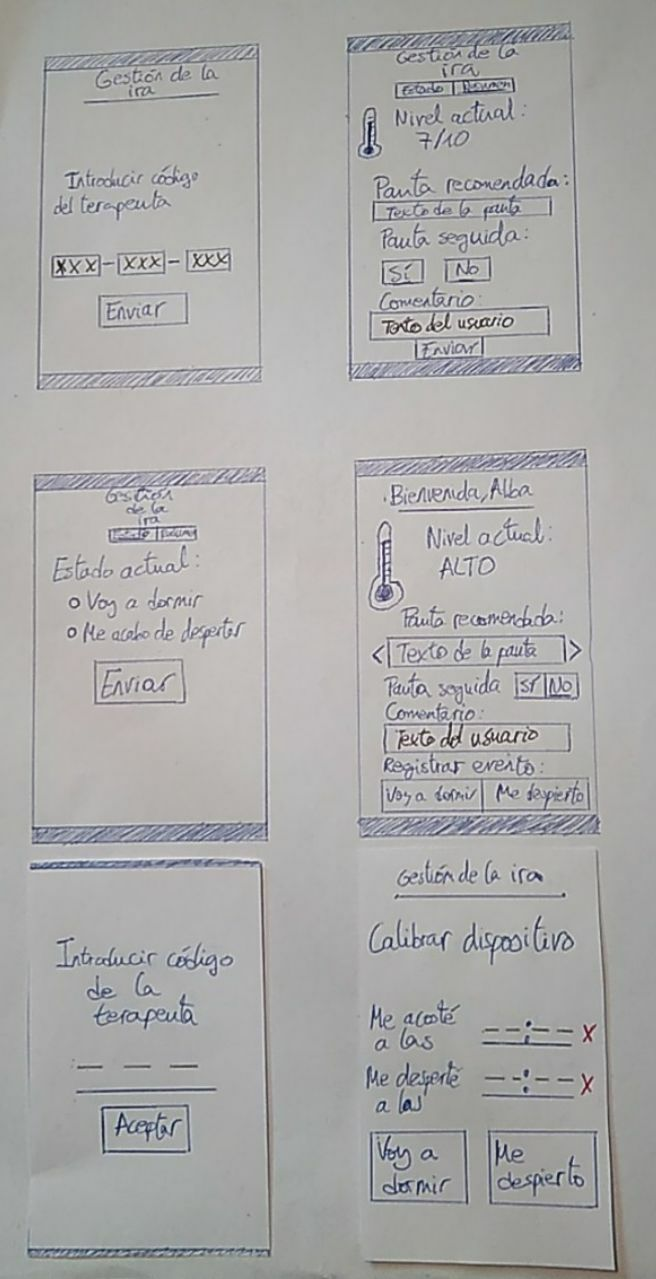
\includegraphics[scale=0.6]{Imagenes/anxA1.jpg}
    \caption[Mockups de la interfaz para el móvil de la fase 2]{Mockups de la interfaz para el móvil de la fase 2}
    \label{fig:mockup1}
\end{figure}

\paragraph{}
Tras realizar la entrevista con la terapeuta apoyados con este mockup, las principales conclusiones que se obtuvo de esta reunión fueron las siguientes:
\begin{itemize}
    \item La manera de emparejar la pulsera y el paciente es apropiada.
    \item Es importante que el paciente pueda cambiar de pauta si esta no le es útil.
    \item El comentario de las pautas debe ser opcional y se debe poder añadir usando la voz. Esto no ha supuesto ningún cambio en la aplicación puesto que Android ya cuenta con un dictado de voz incorporado.
    \item La manera de calibrar el dispositivo tanto del cuatro y sexto recuadro de la figura~\ref{fig:mockup1} son apropiadas.
    \item Para indicar el grado de ira, es mejor hacerlo con palabras (es decir, como en el segundo recuadro) que de manera numérica (como en el cuarto recuadro).
    \item Los estados que discreticen el grado de ira que verá el paciente deberán ser reducidos para que el paciente pueda identificar su cardinalidad y dimensión con facilidad. Así, la solución se limitará a cinco estados.
    \item Como complemento visual a estas palabras que indican el nivel de ira, el termómetro es una buena opción, pero deberá aparecer en horizontal, estando el menor nivel de ira a la izquierda y el mayor en el otro extremo del termómetro, siguiendo la direccionalidad de la lectura en castellano.
    \item Cuando varíe el grado de ira en el termómetro, no solo debe variar cuánto de lleno se encuentra éste, sino también su color.
    \item La terapeuta indicó que, tal y como comenta Valdez\citeyear{valdez1994effects}, existe una relación estrecha entre emociones y colores, por lo que establecer por ejemplo que el rojo es el estado de calma y el verde es el estado de mayor percepción de la ira es un cambio significativo respecto a la asociación opuesta. En estudios experimentales se ha podido comprobar que los colores de mayor longitud de onda como son el rojo o el amarillo provocan mayor arousal que otros de menor longitud de onda como es el verde. A su vez, Jacobs y Sues  \citeyear{jacobs1975effects} han comprobado en un estudio con los colores rojo, amarillo, verde y azul que existe una mayor asociación del estrés con los colores rojo y amarillo respecto al verde y el azul. Así, a la hora de representar los colores asociados a cada nivel de ira, los colores asociados a estos niveles deberían ser (de menor a mayor nivel de ira): verde < verde-amarillo < amarillo < amarillo-rojo < rojo.
    \item Se deben incluir elementos sonoros que incrementen su volumen en función del nivel de ira del paciente para que este pueda ser consciente de que ha aumentado su nivel de ira.
    \item Se debe incluir en la pantalla de la gestión de la ira de la figura~\ref{fig:mockup1} un elemento para poder seleccionar de manera genérica el tipo de situación que ha generado la ira.
\end{itemize}

\subsubsection{Diseño web}
\paragraph{}
Este es el diseño de la web que utilizarán los terapeutas. A continuación se incluyen los distintos recortables de esta parte del mockup y el desglose de sus elementos.
\begin{itemize}
    \item El elemento de la figura~\ref{fig:mockup2} sirve para mostrar cómo sería el inicio de sesión por si acaso la terapeuta necesitase algún tipo de acceso especial.
    \item El elemento de la figura~\ref{fig:mockup3} muestra una pantalla estándar para registrar a un paciente. El combo para seleccionar el grupo finalmente fue descartado.
    \item El elemento de la figura~\ref{fig:mockup4} muestra cómo se crearían grupos y se modificaría su composición de pacientes. Estos grupos más adelante se podrían utilizar para tener agrupadas las pautas asociadas.
    \item En la figura~\ref{fig:mockup5} se muestran dos alternativas para mostrar las pautas: una única tabla para todos los niveles de activación en la que se cuenta con una columna del porcentaje de efectividad general entre los pacientes y una segunda con el texto de la pauta. La primera opción es más visual y cuenta con menos información: no se incluye la columna del porcentaje de éxito de cada pauta y las pautas están divididas en tablas según el nivel de activación asociado\footnote{En caso de que una pauta pueda utilizarse para varios niveles de activación, esta aparecerá replicada en ambas tablas}.
    \item En la figura~\ref{fig:mockup6} aparece una pantalla genérica para modificar el paciente en la que a su vez aparece la información asociada a las pautas que le han ido apareciendo en la aplicación móvil.
    \item En la figura~\ref{fig:mockup7} aparecen las tres opciones que se presentaban a la terapeuta para cada paciente en el que se podía ver el resumen de episodios de cada paciente. Dos de ellos consisten en tablas en las que en una aparece las pautas que se recomendaban y en el otro si la pauta suministrada funcionó o no. La opción alternativa era mostrar una gráfica con los distintos episodios acaecidos en un periodo de tiempo que se podía filtrar con el segundo componente de la figura~\ref{fig:mockup9}. De las tres opciones, esta es la que más convenció a la terapeuta, aunque no quedó claro si prefería una gráfica combinada de episodios ponderados o la separación de los episodios por nivel de activación, como aparece en esta gráfica.
    \item En la figura~\ref{fig:mockup8} aparece un elemento genérico para incluir en la cabecera de la pantalla del usuario con información básica sobre este. Al pulsar sobre el botón modificar, se redireccionaría la a pantalla de la figura~\ref{fig:mockup3}.
    \item En la figura~\ref{fig:mockup9} aparecen los dos elementos que se utilizarían tanto en la pantalla principal con el resumen de alertas de todos los pacientes como en la pantalla particular de cada paciente. El botón \textit{ver detalles} tendría por detrás una función javascript para desplazar la vista de la web a aquella en la que se encuentre la tabla o gráfica con el resumen de episodios citados.
    \item En la figura~\ref{fig:mockup10} aparece el resumen de los episodios de todos los pacientes en el periodo especificado en el segundo elemento de la figura anterior. Así, el elemento más a la izquierda sería un filtro de pacientes similar al que se encuentra en páginas web de compra de artículos en la que se podría filtrar a los mismos en función de la información que se tiene de ellos, así como se podría hacer usando el buscador horizontal que se encuentra en la parte superior de la imagen. Al pulsar sobre cualquiera de estas filas, se abriría la página con el resumen de episodios del paciente seleccionado. La diferencia entre ambas tablas reside principalmente en la utilización del espacio y en que la información provista sea menos o más visual: la opción más a la izquierda, a diferencia de lo que ocurre con la opción de la derecha, no incluiría fotografía y estaría pensada para ocupar menos espacio vertical por registro, lo que permitiría poder representar más registros en el mismo espacio respecto a la segunda opción.
    \item En la figura~\ref{fig:mockup11} aparece el resumen de los episodios para todos los pacientes. Esto se incluiría en la página principal. La información es la misma, lo único que varía es su representación.
\end{itemize}

\begin{figure}[!htbp]
    \centering
    %width=3cm, height=3cm
    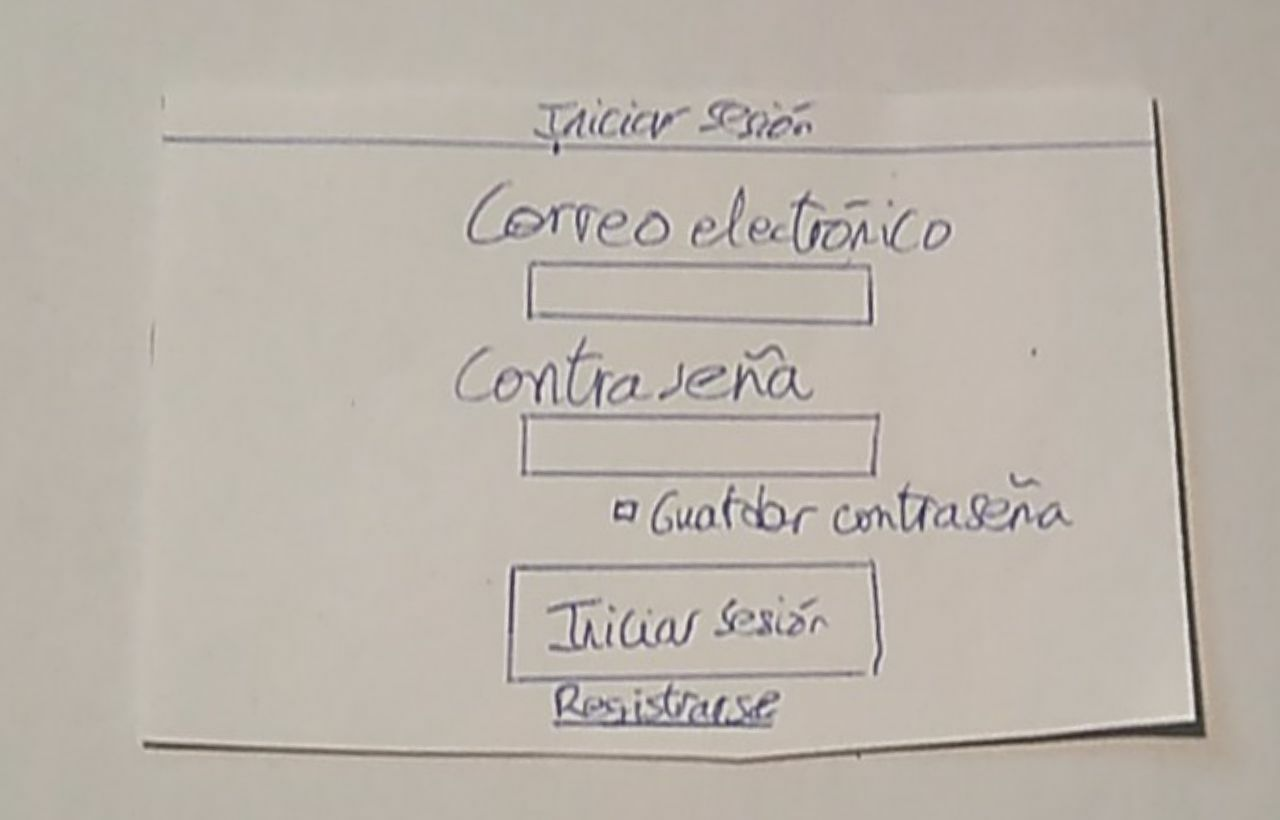
\includegraphics[scale=0.3]{Imagenes/anxA2.jpg}
    \caption[Mockup de la interfaz para la web de la fase 1 (I)]{Mockup de la interfaz para la web de la fase 2 (I)}
    \label{fig:mockup2}
\end{figure}

\begin{figure}[!htbp]
    \centering
    %width=3cm, height=3cm
    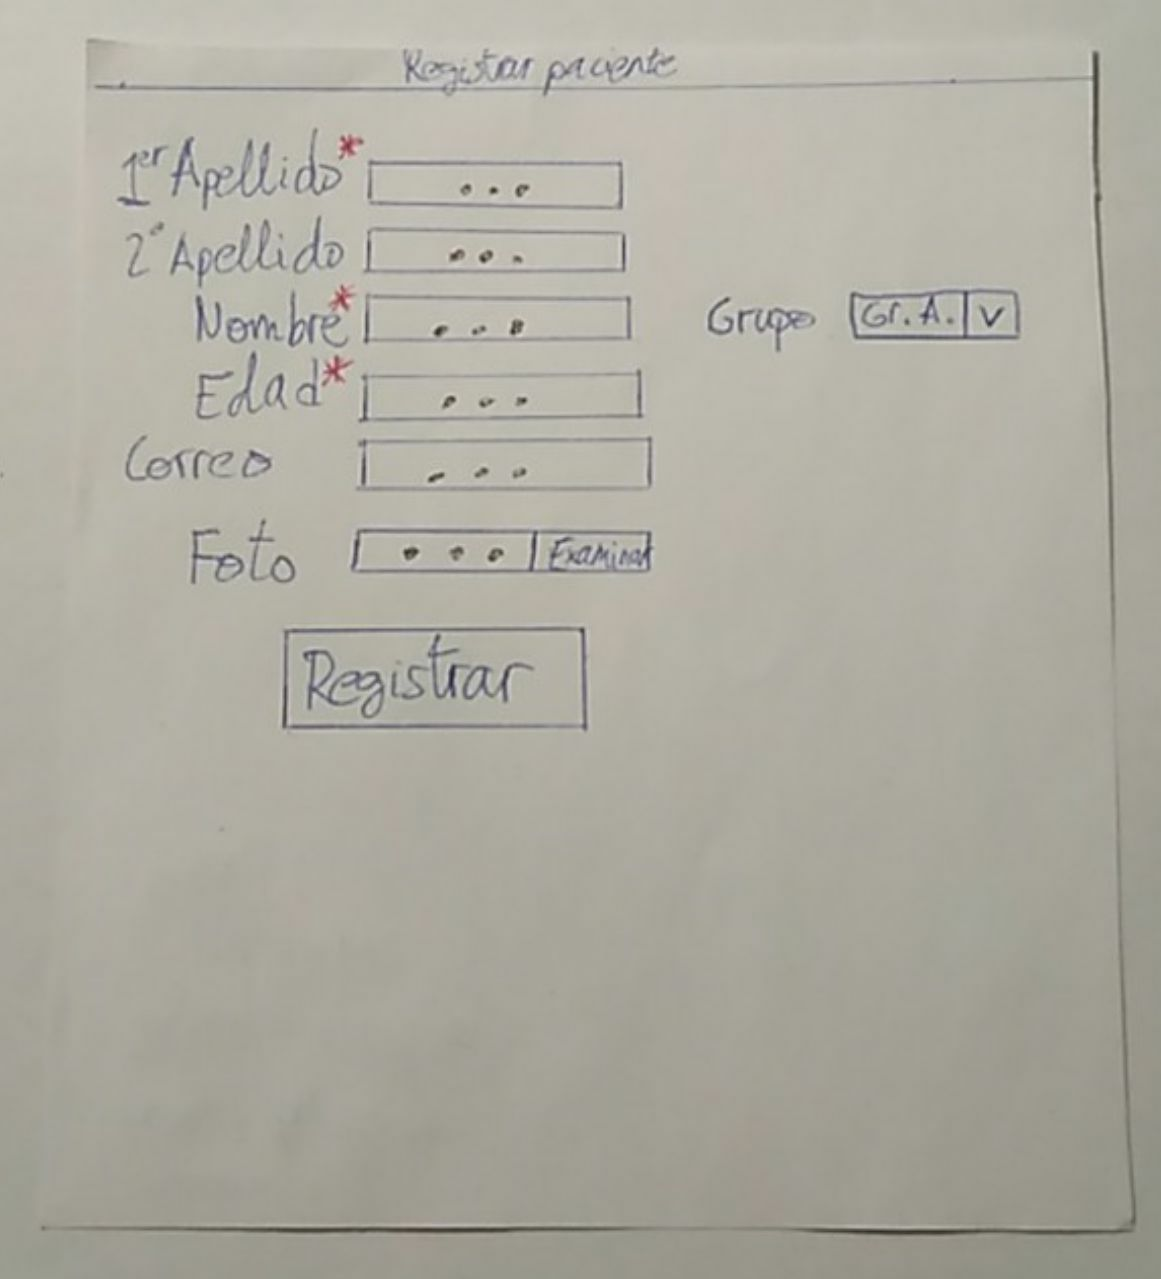
\includegraphics[scale=0.3]{Imagenes/anxA3.jpg}
    \caption[Mockup de la interfaz para la web de la fase 1 (II)]{Mockup de la interfaz para la web de la fase 2 (II)}
    \label{fig:mockup3}
\end{figure}

\begin{figure}[!htbp]
    \centering
    %width=3cm, height=3cm
    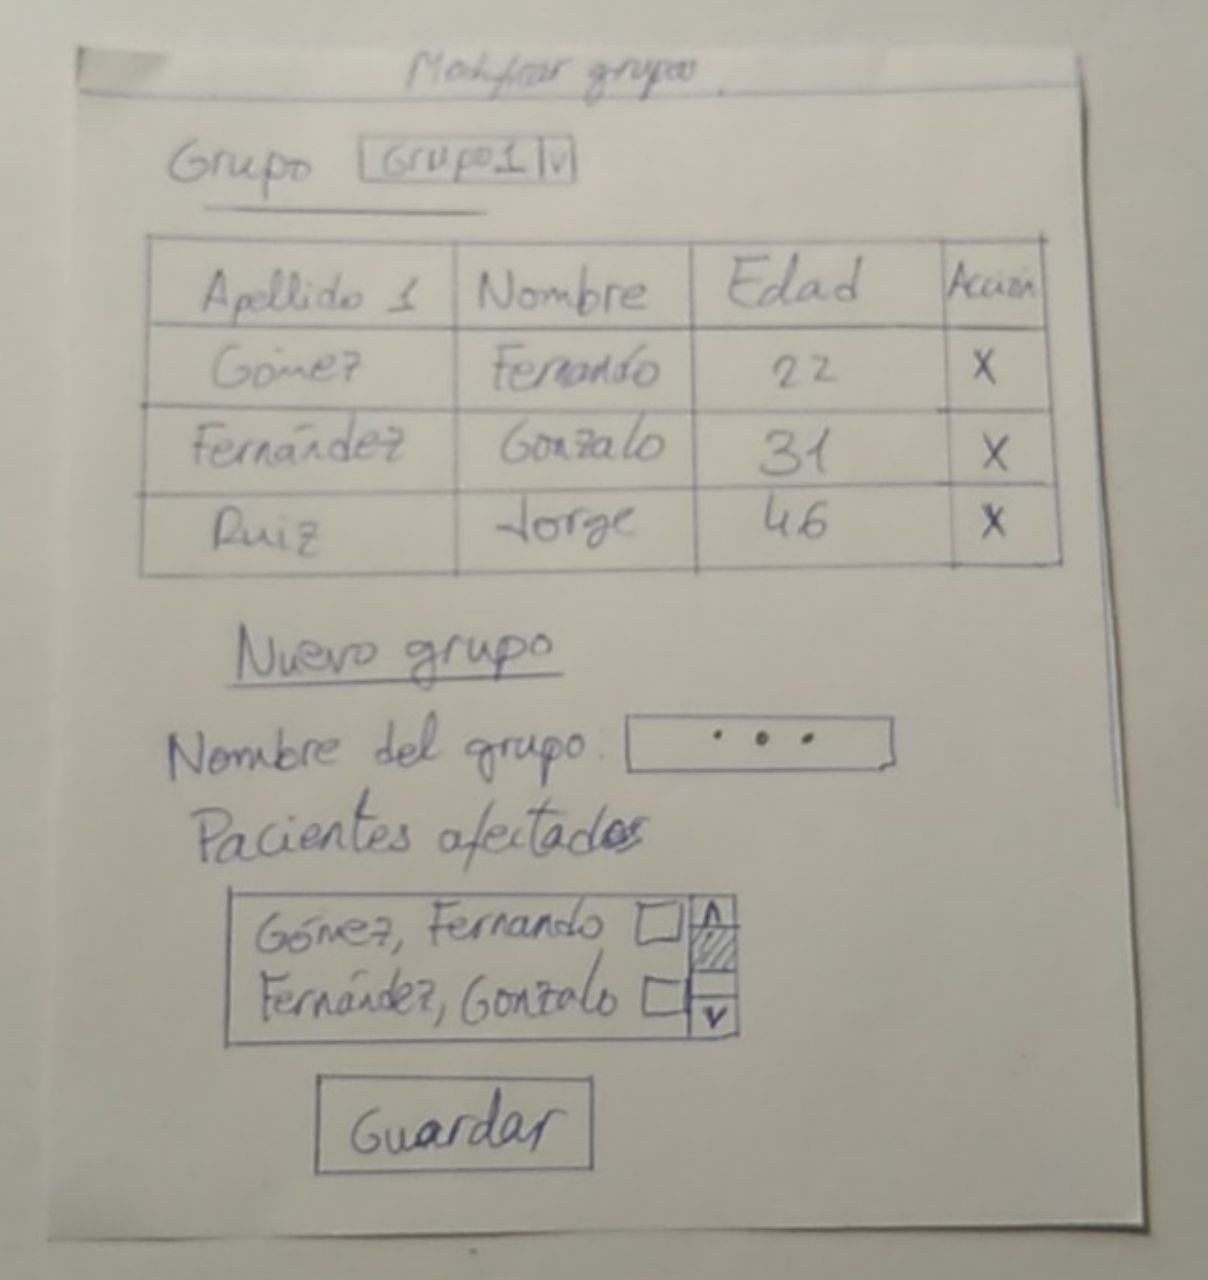
\includegraphics[scale=0.3]{Imagenes/anxA4.jpg}
    \caption[Mockup de la interfaz para la web de la fase 1 (III)]{Mockup de la interfaz para la web de la fase 2 (III)}
    \label{fig:mockup4}
\end{figure}

\begin{figure}[!htbp]
    \centering
    %width=3cm, height=3cm
    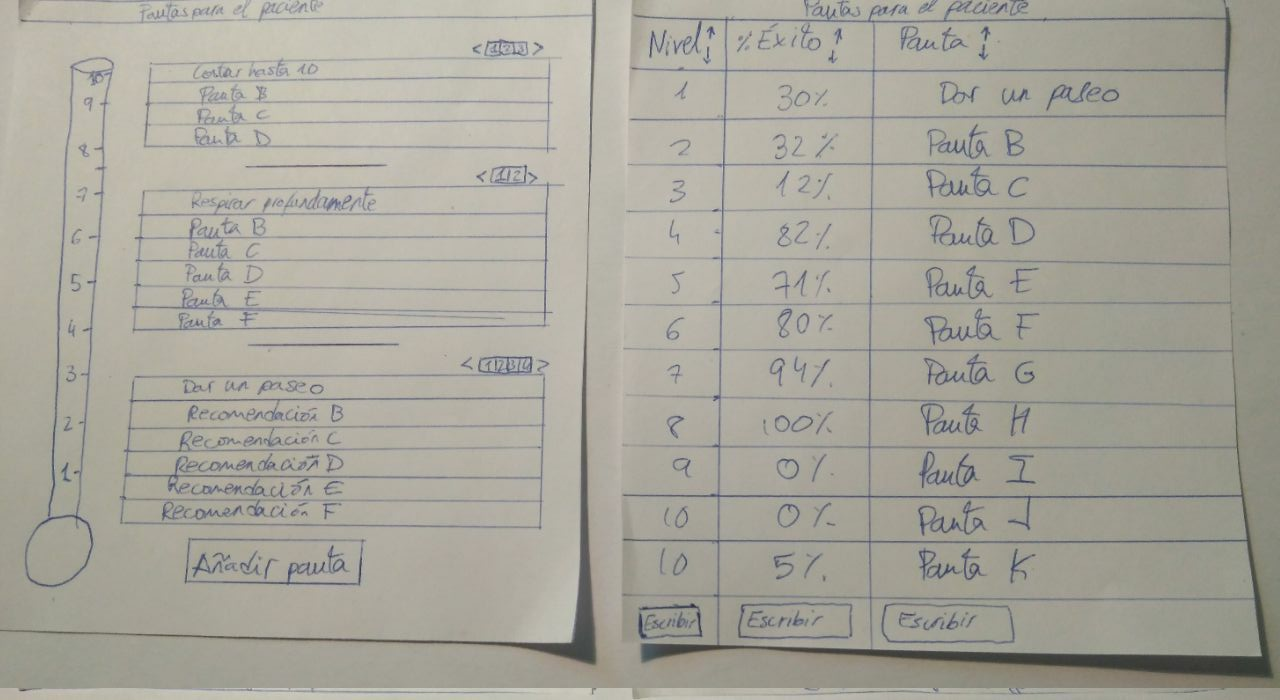
\includegraphics[scale=0.3]{Imagenes/anxA5.jpg}
    \caption[Mockup de la interfaz para la web de la fase 1 (IV)]{Mockup de la interfaz para la web de la fase 2 (IV)}
    \label{fig:mockup5}
\end{figure}

\begin{figure}[!htbp]
    \centering
    %width=3cm, height=3cm
    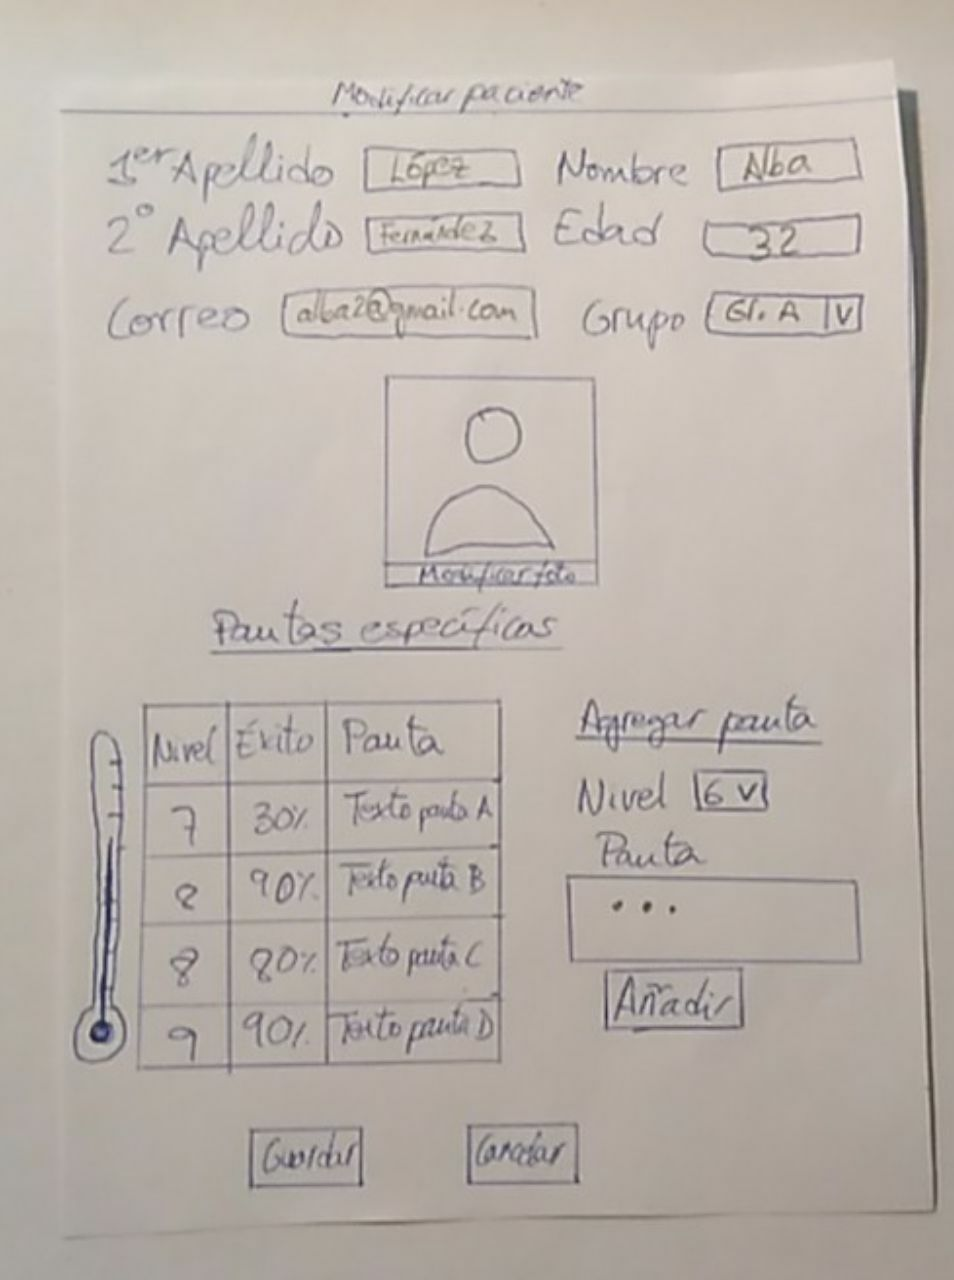
\includegraphics[scale=0.3]{Imagenes/anxA6.jpg}
    \caption[Mockup de la interfaz para la web de la fase 1 (V)]{Mockup de la interfaz para la web de la fase 2 (V)}
    \label{fig:mockup6}
\end{figure}

\begin{figure}[!htbp]
    \centering
    %width=3cm, height=3cm
    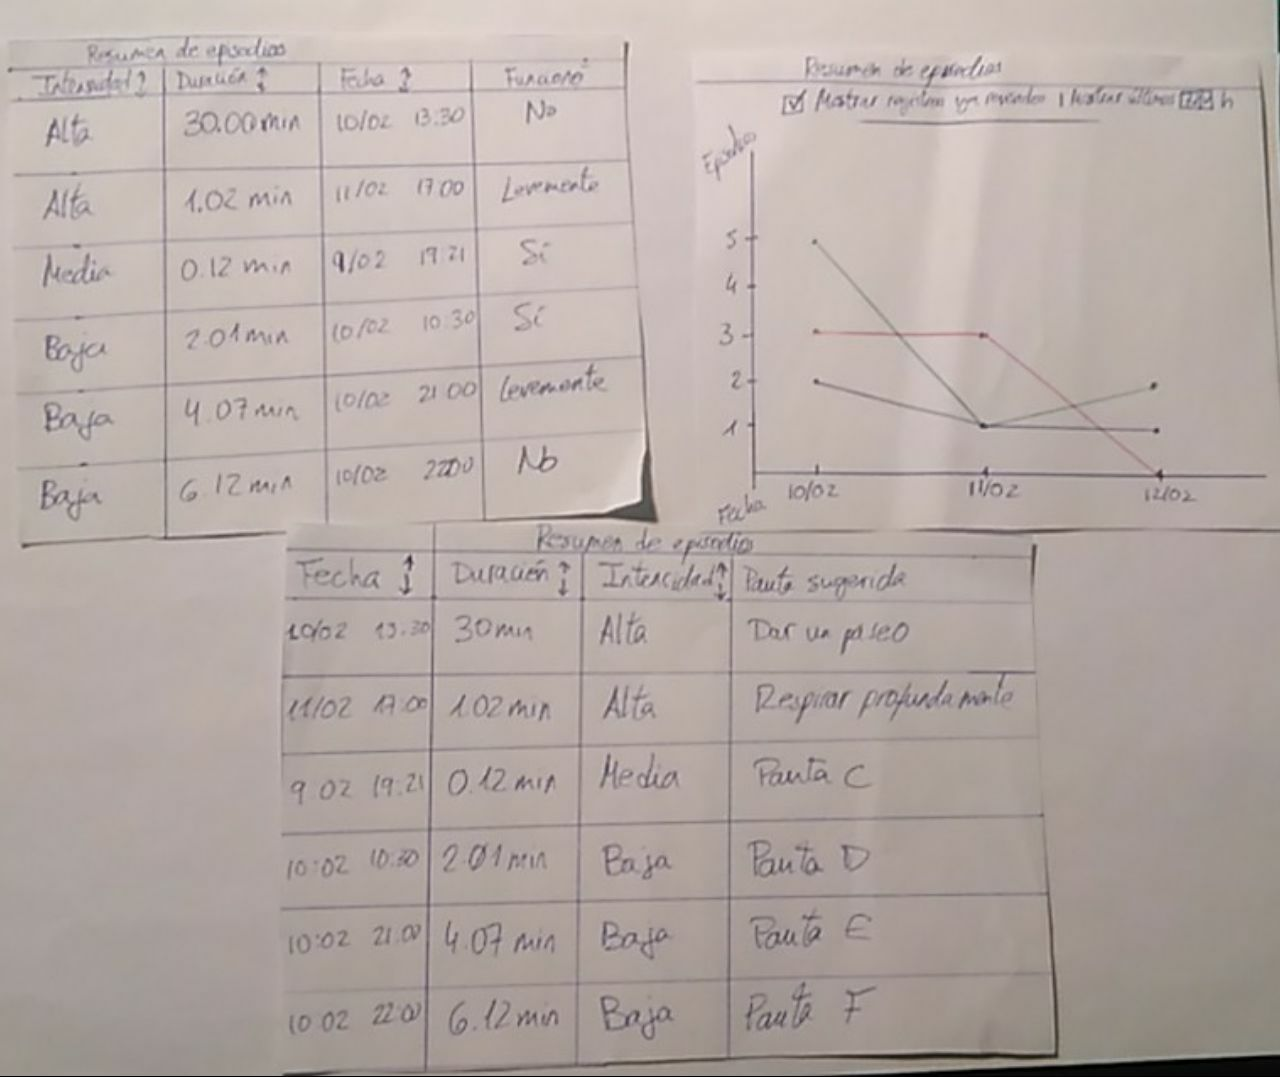
\includegraphics[scale=0.3]{Imagenes/anxA7.jpg}
    \caption[Mockup de la interfaz para la web de la fase 1 (VI)]{Mockup de la interfaz para la web de la fase 2 (VI)}
    \label{fig:mockup7}
\end{figure}

\begin{figure}[!htbp]
    \centering
    %width=3cm, height=3cm
    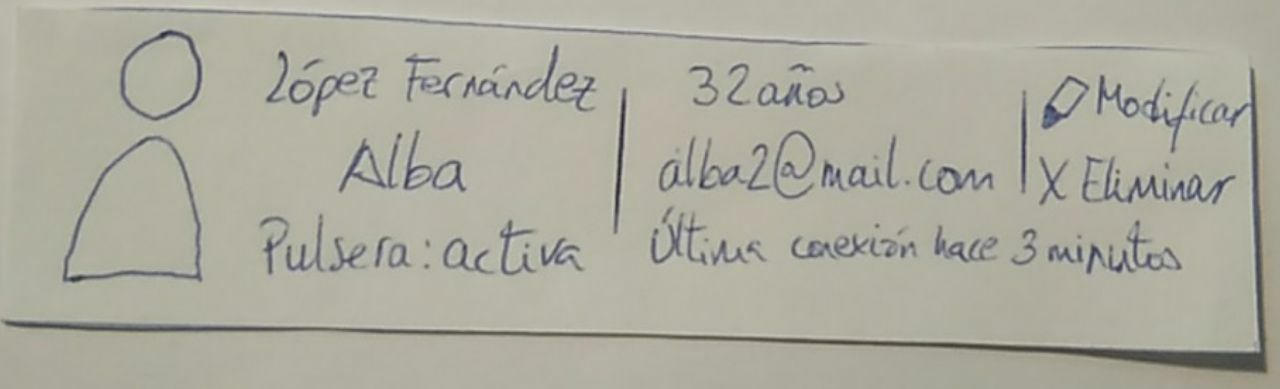
\includegraphics[scale=0.3]{Imagenes/anxA8.jpg}
    \caption[Mockup de la interfaz para la web de la fase 1 (VII)]{Mockup de la interfaz para la web de la fase 2 (VII)}
    \label{fig:mockup8}
\end{figure}

\begin{figure}[!htbp]
    \centering
    %width=3cm, height=3cm
    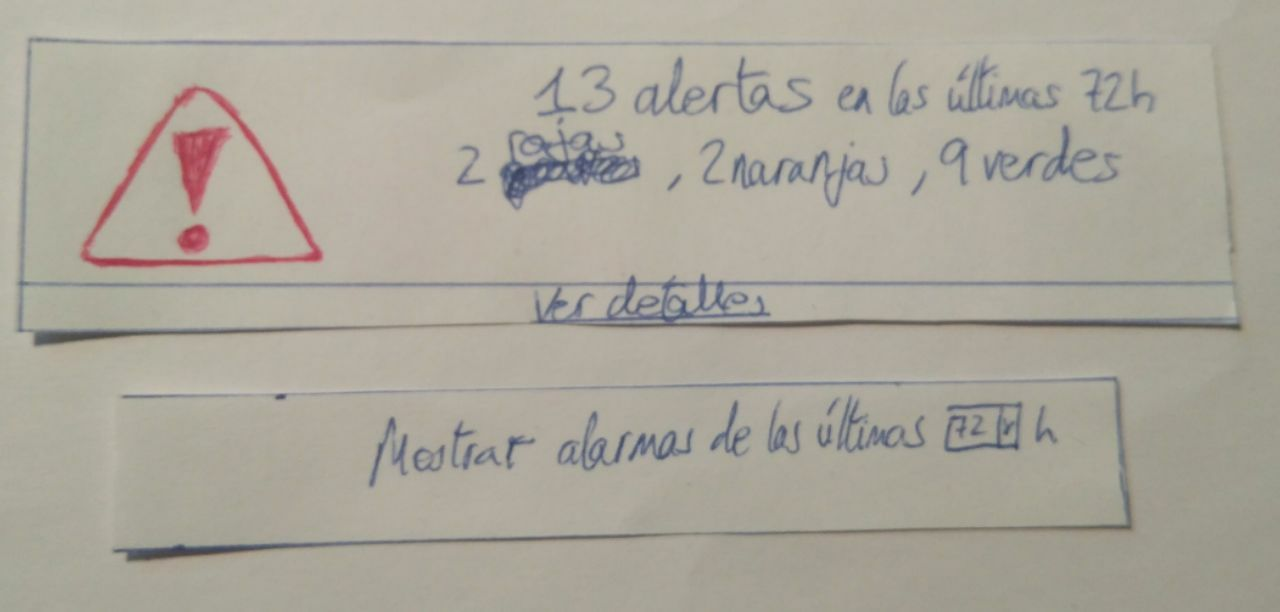
\includegraphics[scale=0.3]{Imagenes/anxA9.jpg}
    \caption[Mockup de la interfaz para la web de la fase 1 (VIII)]{Mockup de la interfaz para la web de la fase 2 (VIII)}
    \label{fig:mockup9}
\end{figure}

\begin{figure}[!htbp]
    \centering
    %width=3cm, height=3cm
    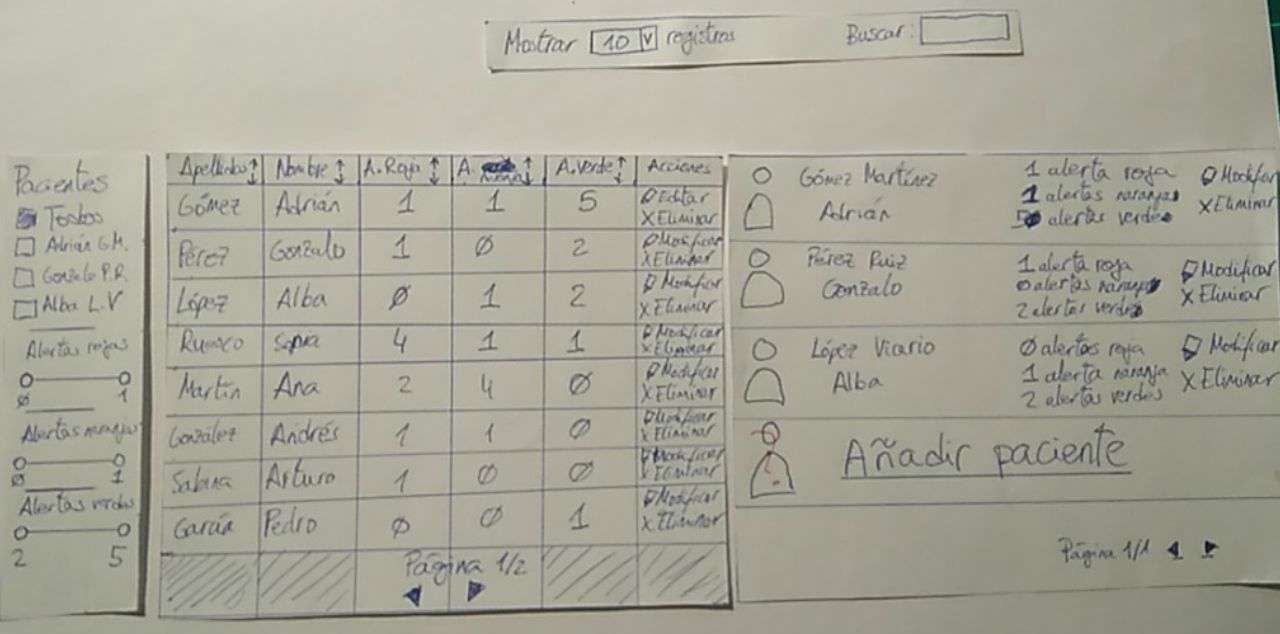
\includegraphics[scale=0.3]{Imagenes/anxA10.jpg}
    \caption[Mockup de la interfaz para la web de la fase 1 (IX)]{Mockup de la interfaz para la web de la fase 2 (IX)}
    \label{fig:mockup10}
\end{figure}

\begin{figure}[!htbp]
    \centering
    %width=3cm, height=3cm
    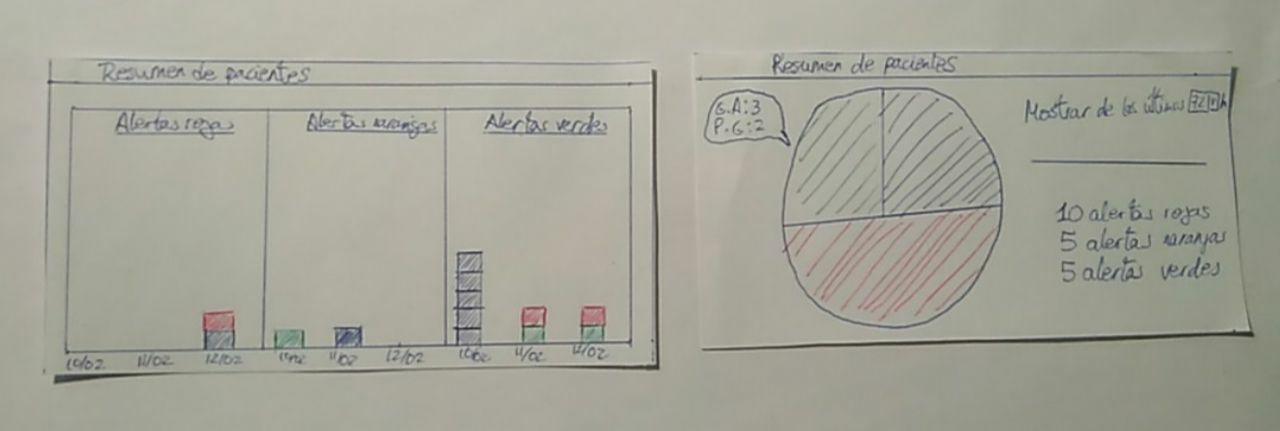
\includegraphics[scale=0.3]{Imagenes/anxA11.jpg}
    \caption[Mockup de la interfaz para la web de la fase 1 (X)]{Mockup de la interfaz para la web de la fase 2 (X)}
    \label{fig:mockup11}
\end{figure}

\paragraph{}
Tras realizar la entrevista con la terapeuta apoyados con este mockup, las principales conclusiones que se obtuvo de esta reunión fueron las siguientes:

\begin{itemize}
    \item El método de autentificación del terapeuta con la tupla correo electrónico y contraseña es apropiado.
    \item Es apropiado poder incluir las fotos de pacientes para mejorar la visualización. El correo electrónico no es necesario y el grupo al que pertenece cada paciente es prescindible. Para futuras versiones podría ser interesante agrupar a los pacientes y obtener resultados globales de estos grupos pero para esta versión se acaba decidiendo que es mejor centrarse en una solución más sencilla. Por ello, la figura~\ref{fig:mockup3} debe suprimir la selección del grupo y la pantalla de la figura~\ref{fig:mockup4} no tiene que aparecer.
    \item Entre el primer y segundo elemento de la figura~\ref{fig:mockup4} para representar las pautas de cada paciente, se considera que la solución tiene que ser algo intermedio: conservar la estructura del primer elemento de dividir las pautas en diversas tablas según su grado de intensidad (con un termómetro en paralelo para poder correlacionar fácilmente la intensidad de cada pauta) pero añadiendo columnas adicionales a las pautas como por ejemplo el porcentaje de éxito, tal y como se ve en el segundo elemento.
    \item Se considera apropiado que en el resumen de los episodios de ira figure el tiempo que se mantuvo el paciente en cada uno de los estados, tal y como aparece en el primer elemento de la figura~\ref{fig:mockup7}.
    \item La información de la pauta recomendada para cada episodio, tal y como aparece en el tercer elemento de la figura~\ref{fig:mockup7} se considera apropiada, pero es incompleto, ya que para un mismo estado al paciente se le puede haber recomendado más de una pauta. El paciente puede haber descartado pautas previas, y esta información es importante que quede registrada.
    \item El segundo elemento de la figura~\ref{fig:mockup7} representa los episodios en formato histograma, lo que es correcto. El gráfico de tarta que aparece en el segundo elemento de la gráfica ~\ref{fig:mockup11} no aporta información útil, porque cómo se ha desarrollado el episodio es relevante, como por ejemplo el tiempo que ha pasado en cada estado. El segundo elemento de la figura~\ref{fig:mockup7} hace una aproximación a esto pero es incompleto, puesto que es necesario que sea una gráfica interactiva que permita poder ampliarla para por ejemplo poder seleccionar solo un episodio e ir viéndolos uno a uno. Para este fin, la terapeuta propone basarse en el ejemplo de las gráficas de los desfibriladores.
    \item Las figuras~\ref{fig:mockup8} y ~\ref{fig:mockup9} son elementos adicionales que sirven para decorar las pantallas que se iban generando. La figura~\ref{fig:mockup8} se considera apropiada mientras que el primer elemento de la figura~\ref{mockup9} se considera que no aporta información útil para la terapeuta.
    \item En la figura~\ref{fig:mockup10} aparecen dos modelos de tablas y una serie de filtros para poder buscar los pacientes en dichas tablas. Los filtros se consideran apropiados, y ambos formatos de tablas también a excepción de las columnas que indican el número de alertas de cada una de las intensidades de la ira de cada paciente, ya que esta información sin estar agrupada en episodios y desglosada en fechas, no aporta información relevante al terapeuta.
\end{itemize}

\subsection{Segundo diseño: mockups generados con las herramientas finales}
\paragraph{}
Para este diseño, se han utilizado las mismas herramientas que se pretendían usar durante la implementación de la solución para que así el diseño que se muestre pueda ser replicado de manera prácticamente idéntica a lo que se muestre a la terapeuta. Es decir, estará implementado el \textit{Front-end} de la aplicación, y, si los elementos son validados, en la implementación final a estos se les añadiría el \textit{Back-end} correspondiente.

\subsubsection{Diseño móvil}

\paragraph{}
Las pantallas de esta fase para el móvil son las siguientes:

\begin{itemize}
    \item En la figura~\ref{fig:mockup12} aparece la pantalla para introducir el código para sincronizar la pulsera y el móvil con el paciente. Es la equivalente de la fase anterior que aparece en la figura~\ref{fig:mockup1}.
    \item En la figura~\ref{fig:mockup13} podemos ver la pantalla para sincronizar el dispositivo durante su primer uso.
    \item En la figura~\ref{fig:mockup14} encontramos la que será la pantalla principal, donde aparece la pauta recomendada, el nivel de la ira representado mediante un termómetro horizontal, la posibilidad de cambiar de pauta y de enviar comentarios sobre la pauta en cuestión.
    \item En la figura~\ref{fig:mockup15} se encuentra una pantalla de resumen de la evolución seguida por el paciente. Esto es una innovación respecto a la anterior versión puesto que la terapeuta comentó que esta información puede servir para motivar al paciente al poder verificar en un histograma cómo se han reducido sus episodios de ira.
    \item En la figura~\ref{fig:mockup16} podemos ver la manera que se utilizaría para cambiar entre las pantallas. En lugar de tener un menú horizontal que quite espacio para el resto de pantallas, este menú se desplegará como se hace en aplicaciones como Telegram o Whatsapp mediante el pulsado en un bocadillo a la izquierda de la barra horizontal superior o mediante el desplazamiento de la pantalla de izquierda a derecha.
\end{itemize}

\begin{figure}[!htbp]
    \centering
    %width=3cm, height=3cm
    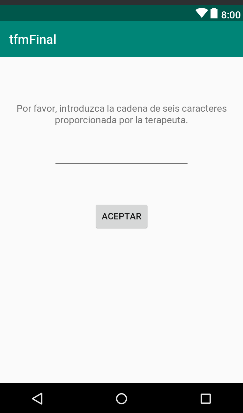
\includegraphics[scale=0.6]{Imagenes/anxA12.png}
    \caption[Mockup de la interfaz para el móvil de la fase 3 (I)]{Mockup de la interfaz para el móvil de la fase 3 (I)}
    \label{fig:mockup12}
\end{figure}

\begin{figure}[!htbp]
    \centering
    %width=3cm, height=3cm
    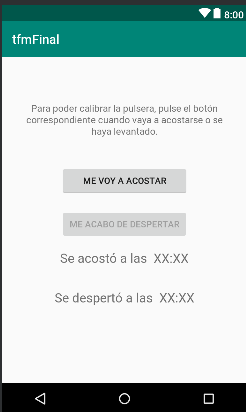
\includegraphics[scale=0.6]{Imagenes/anxA13.png}
    \caption[Mockup de la interfaz para el móvil de la fase 3 (II)]{Mockup de la interfaz para el móvil de la fase 3 (II)}
    \label{fig:mockup13}
\end{figure}

\begin{figure}[!htbp]
    \centering
    %width=3cm, height=3cm
    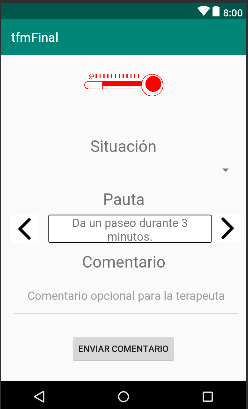
\includegraphics[scale=0.6]{Imagenes/anxA14.png}
    \caption[Mockup de la interfaz para el móvil de la fase 3 (III)]{Mockup de la interfaz para el móvil de la fase 3 (III)}
    \label{fig:mockup14}
\end{figure}

\begin{figure}[!htbp]
    \centering
    %width=3cm, height=3cm
    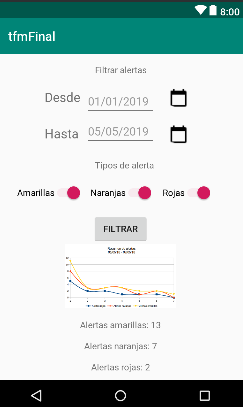
\includegraphics[scale=0.6]{Imagenes/anxA15.png}
    \caption[Mockup de la interfaz para el móvil de la fase 3 (IV)]{Mockup de la interfaz para el móvil de la fase 3 (IV)}
    \label{fig:mockup15}
\end{figure}

\begin{figure}[!htbp]
    \centering
    %width=3cm, height=3cm
    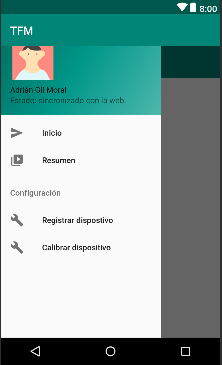
\includegraphics[scale=0.6]{Imagenes/anxA16.png}
    \caption[Mockup de la interfaz para el móvil de la fase 3 (V)]{Mockup de la interfaz para el móvil de la fase 3 (V)}
    \label{fig:mockup16}
\end{figure}

\paragraph{}
Al revisar este diseño con la terapeuta, se obtuvieron las siguientes conclusiones:

\begin{itemize}
    \item Las pantallas que se muestran son correctas, pero sigue fallando el hecho de que se incluye la intensidad de las alertas al paciente. Tanto el paciente como el terapeuta solo tienen que ver episodios, las alertas son parámetros de entrada para generar estos episodios.
    \item El termómetro de la imágen debe ir al revés: el elemento de mayor grosor tiene que ir a la izquierda, que representará el menor nivel de ira.
    \item Se debe incluir un widget en la aplicación en el que aparezca un pequeño termómetro con el nivel de ira del paciente en ese momento.
    \item Se deben incluir mensajes de alertas motivacionales para el paciente para cuando se vea que está progresando y que así tenga un refuerzo positivo.
\end{itemize}

\subsubsection{Diseño web}
\paragraph{}
En este caso, se diseñaron exclusivamente las pantallas que pudieran ser fruto de mayor controversia, eliminando pantallas estándar como las de inicio de sesión o de modificación de pacientes pues la interfaz de estos no debería variar sensiblemente durante estas fases. Dicho esto, las pantallas de esta fase para la web son las siguientes:
\begin{itemize}
    \item En la figura ~\ref{fig:mockup17} podemos ver la pantalla principal, que sería la implementación de los elementos de la figura ~\ref{fig:mockup11}. Como se ve, no se han incluído las gráficas propuestas al no considerarse útiles.
    \item En las figuras ~\ref{fig:mockup18} y ~\ref{fig:mockup19} se puede ver la pantalla en la que aparecería el resumen de cada paciente mediante una gráfica y una tabla de formato acordeón a continuación con información detallada de cada uno de los estados del episodio por los que ha pasado el paciente.
    \item En la figura ~\ref{fig:mockup20} se puede ver la implementación de la pantalla ~\ref{fig:mockup5} en la versión en la que las pautas están separadas por el nivel de activación.
\end{itemize}

\begin{figure}[!htbp]
    \centering
    %width=3cm, height=3cm
    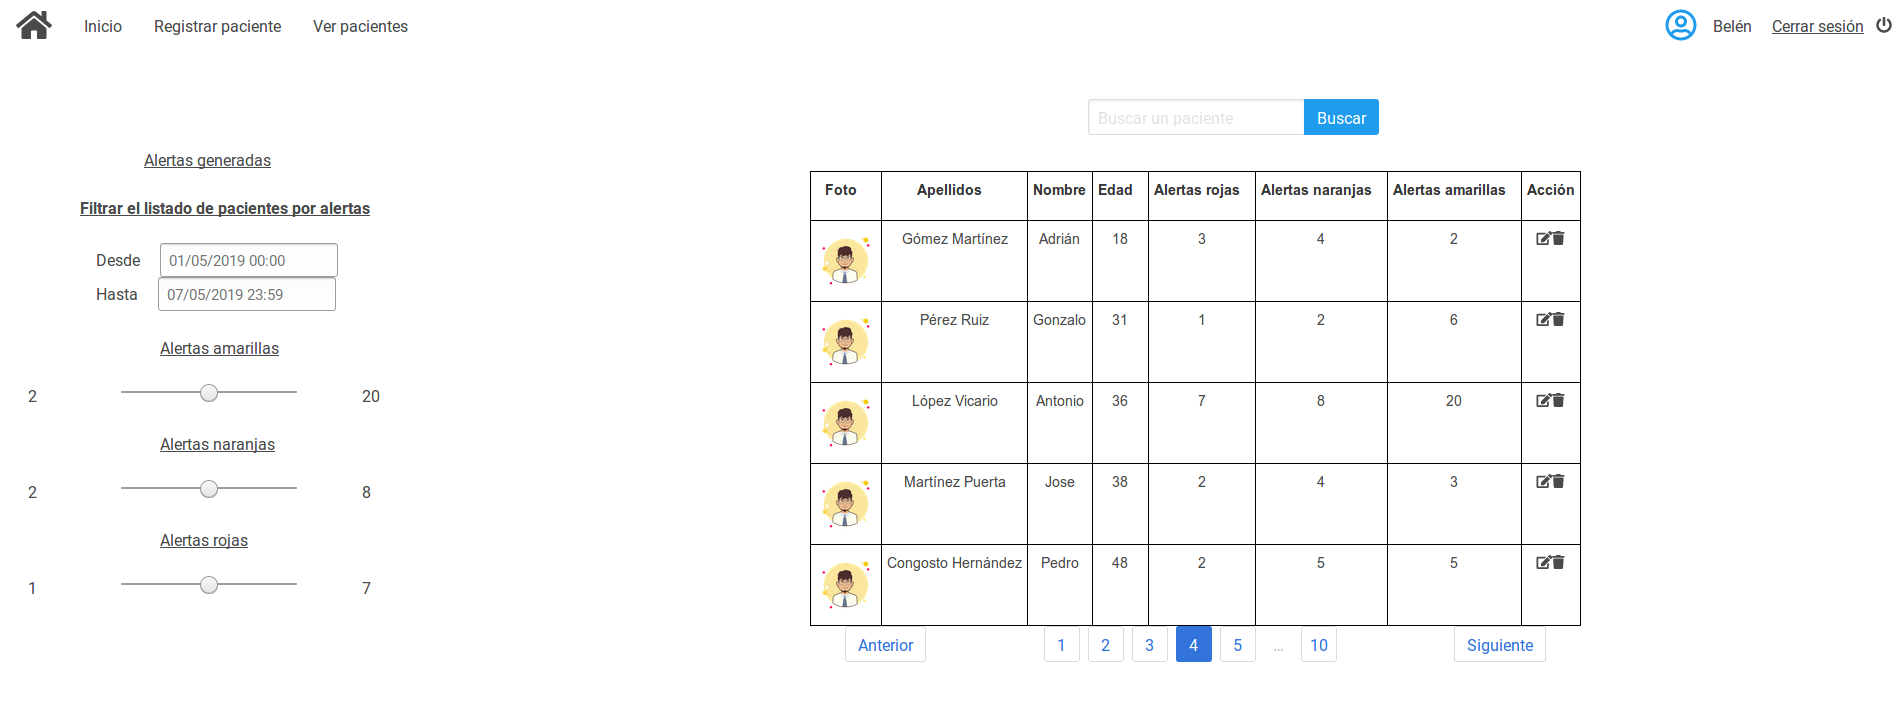
\includegraphics[scale=0.24]{Imagenes/anxA17.png}
    \caption[Mockup de la interfaz para la web de la fase 3 (I)]{Mockup de la interfaz para la web de la fase 3 (I)}
    \label{fig:mockup17}
\end{figure}

\begin{figure}[!htbp]
    \centering
    %width=3cm, height=3cm
    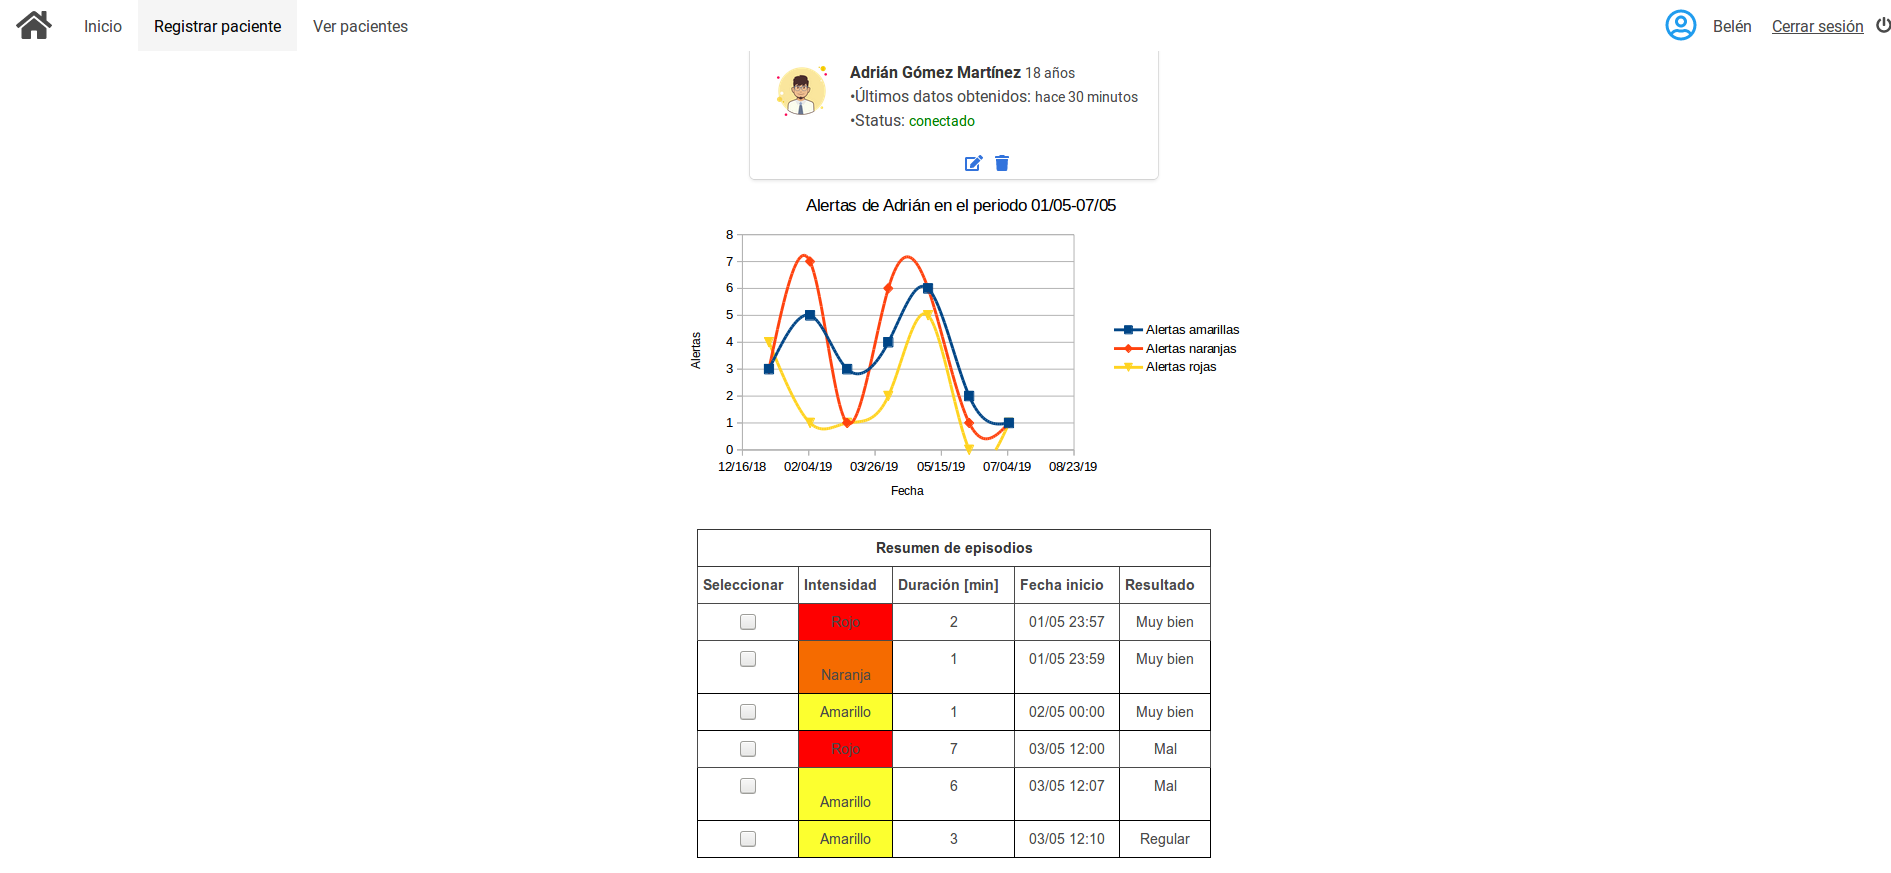
\includegraphics[scale=0.24]{Imagenes/anxA18.png}
    \caption[Mockup de la interfaz para la web de la fase 3 (II-I)]{Mockup de la interfaz para la web de la fase 3 (II-I)}
    \label{fig:mockup18}
\end{figure}

\begin{figure}[!htbp]
    \centering
    %width=3cm, height=3cm
    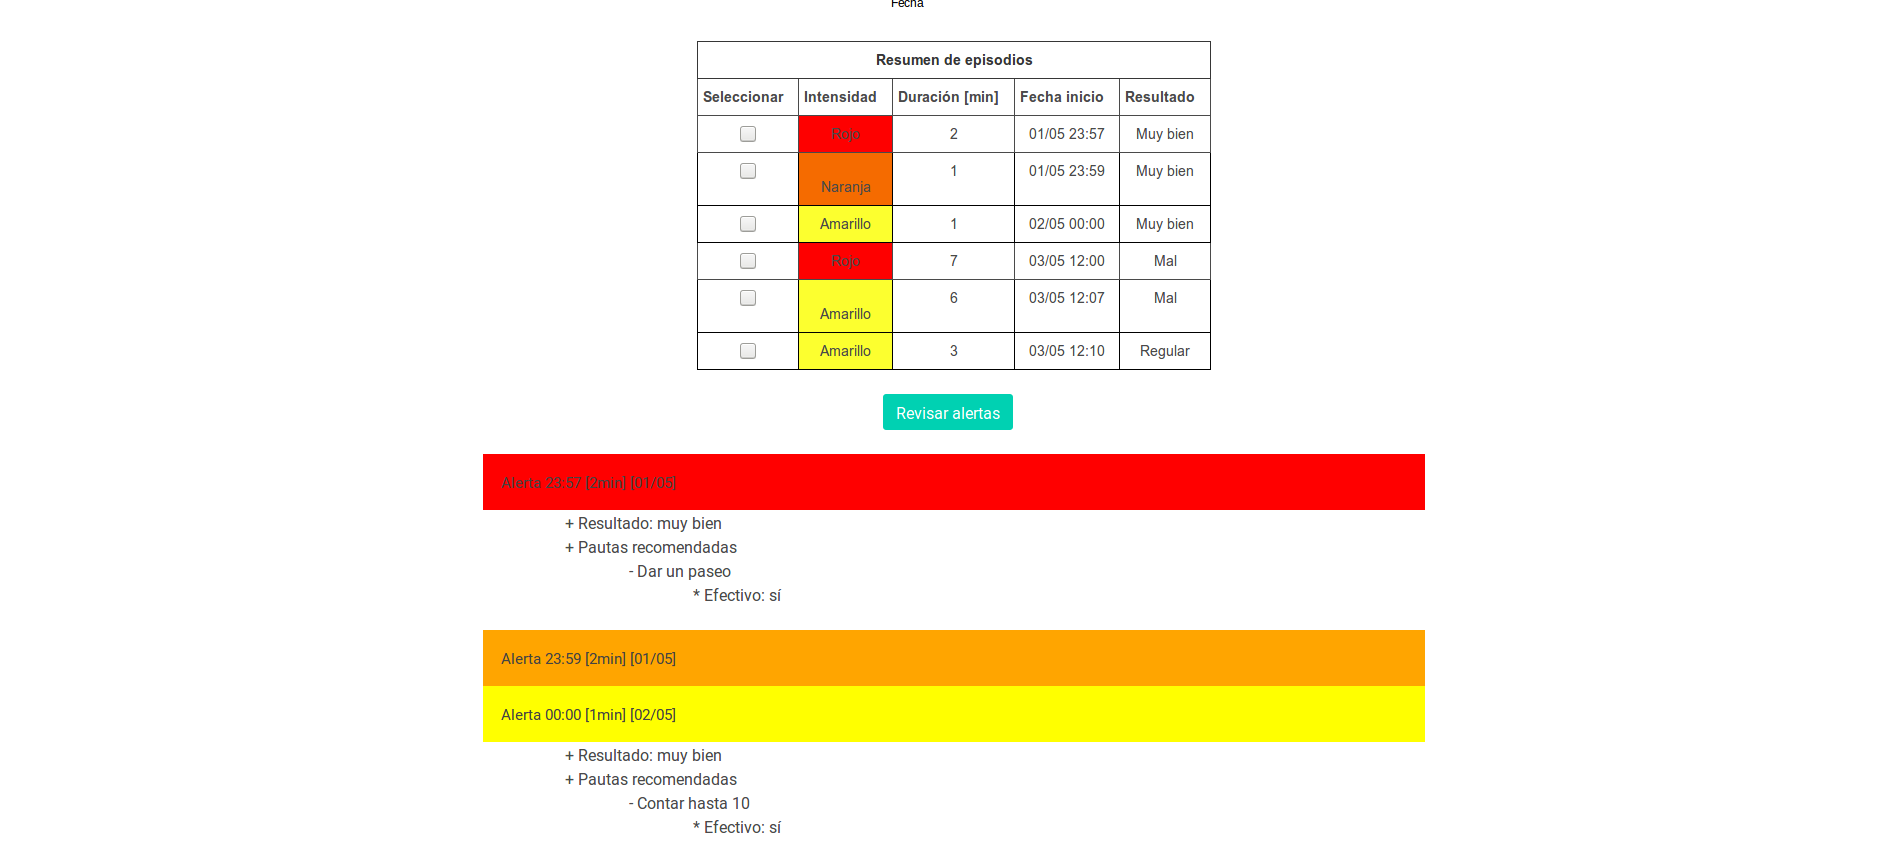
\includegraphics[scale=0.24]{Imagenes/anxA19.png}
    \caption[Mockup de la interfaz para la web de la fase 3 (II-II)]{Mockup de la interfaz para la web de la fase 3 (II-II)}
    \label{fig:mockup19}
\end{figure}

\begin{figure}[!htbp]
    \centering
    %width=3cm, height=3cm
    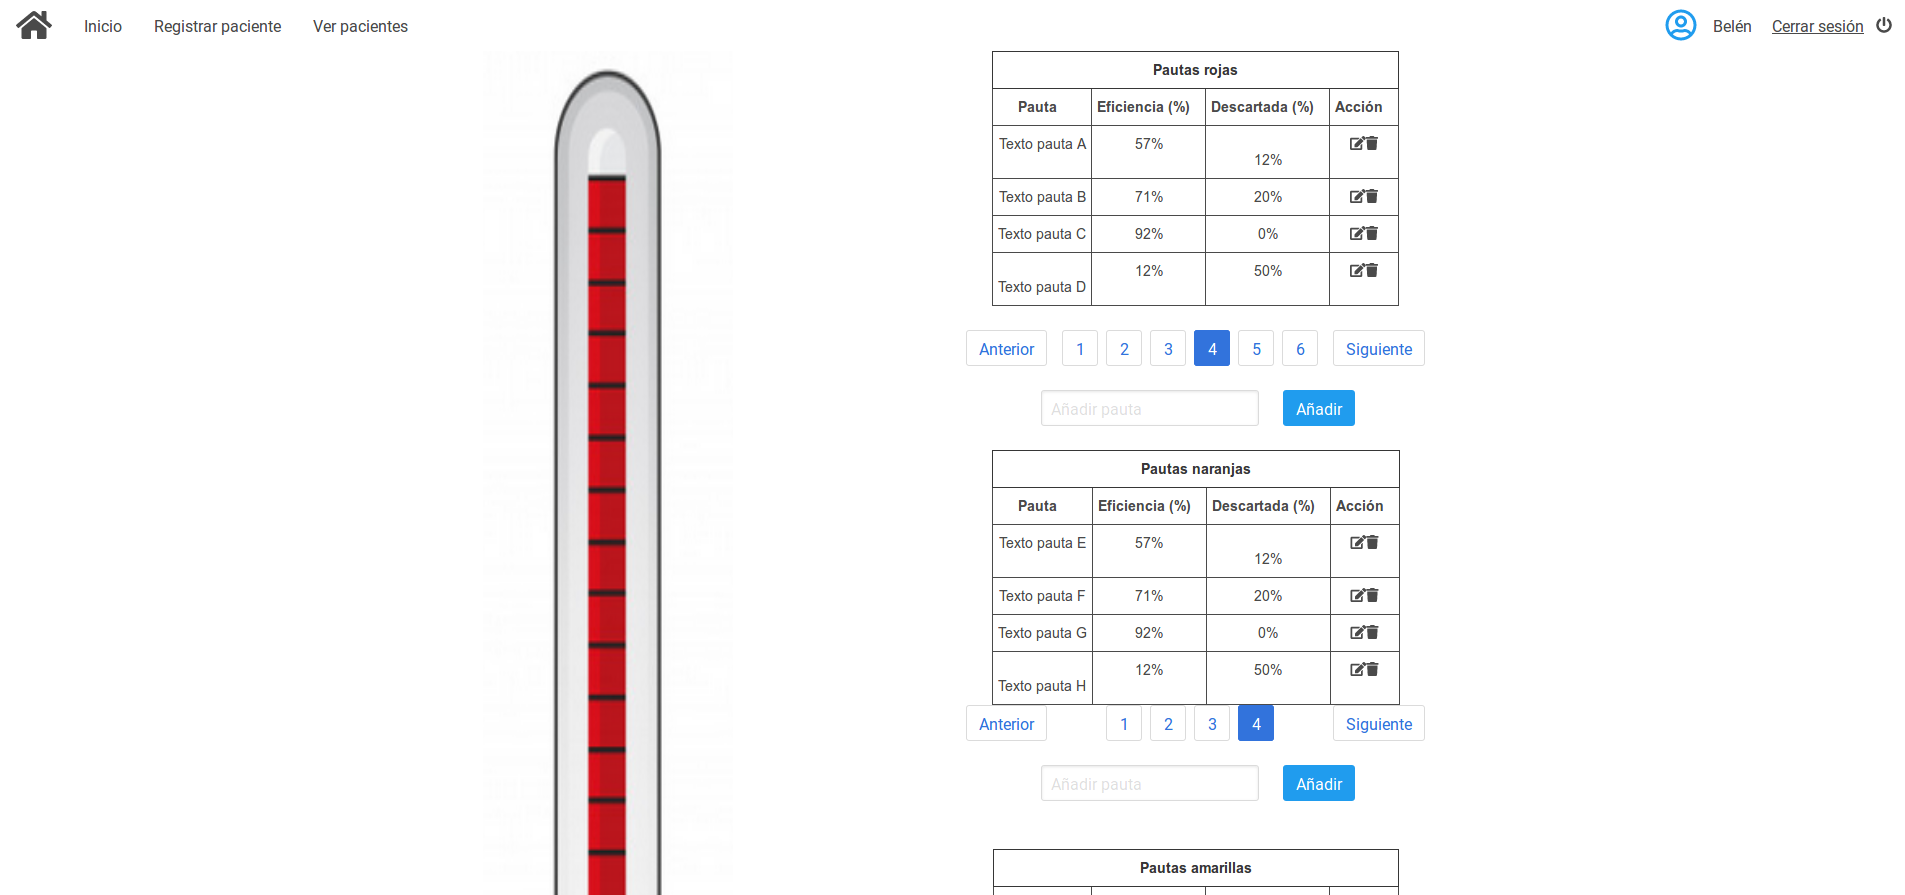
\includegraphics[scale=0.24]{Imagenes/anxA20.png}
    \caption[Mockup de la interfaz para la web de la fase 3 (III)]{Mockup de la interfaz para la web de la fase 3 (II)}
    \label{fig:mockup20}
\end{figure}

\paragraph{}
Tras la reunión con la terapeuta, los puntos que se sacaron en claro fueron los siguientes:

\begin{itemize}
    \item Las pantallas de las figura~\ref{fig:mockup17} y~\ref{fig:mockup18}  siguen teniendo en las tablas y en la gráfica alertas en lugar de eventos, por lo que tiene que actualizarse esta información.
    \item La tabla de la figura~\ref{fig:mockup18} debe ser interactiva. Se insiste en emular el diseño de los desfibriladores. La tabla de la figura~\ref{fig:mockup19} que aparece debajo indicando las pautas seguidas en los distintos momentos es correcta, pero en el diseño final tiene que ser más detallada.
    \item La pantalla de la figura~\ref{mockup20} cumple los objetivos.
    \item Se echa en falta definir la pantalla en la que se añaden las pautas de cada paciente. En estas es necesario crear un sistema para poder heredar pautas de manera grupal para, a partir del paquete de pautas que se ha heredado, poder personalizarlas para cada paciente.
\end{itemize}

%TODO: esto probablemente acabe en otra sección mucho más detallada en la que se expliquen todos los aspectos técnicos de la solución final.
\section{Descripción técnica de la solución}
\paragraph{}
La pulsera es un dispositivo IOT que obtendrá las sensorizaciones del paciente cada [TODO] segundos. Concretamente, obtendrá los datos de sudoración, [TODO: constantes fisiológicas medidas]. Para ello, se ha elegido el modelo [TODO: modelo y descripción del modelo de la pulsera haciendo referencia a la comparación de pulseras del estado del arte].

\paragraph{}
Estas sensorizaciones se enviarán por BLE al dispositivo móvil con sistema operativo Android del paciente. La conexión será gestionada mediante una app creada para este proyecto, que irá guardando las sensorizaciones en una base de datos local de SQLite. La base de datos local estará encriptada con el algoritmo [TODO: rellenar cuando termine la app] para evitar dos posibles ataques: por un lado, si el paciente tiene el móvil \textit{rooteado} y la base de datos no está encriptada, si se instalase una aplicación maligna, esta podría acceder a los datos de la base de datos. Por otro, aunque el paciente no tuviera el móvil \textit{rooteado}, es necesario prevenir que estos datos se vieran expuestos si una tercera persona no autorizada tuviera acceso físico al mismo por ejemplo porque hubiese dejado desatendido su dispositivo temporalmente o le robasen el dispositivo.

\paragraph{}
En las aplicaciones móviles es crucial optimizar al máximo el uso de recursos para evitar que la aplicación creada interfiera con el normal funcionamiento del dispositivo ralentizándolo, consumiendo muchos datos o almacenando datos innecesarios. En esta línea, la aplicación borrará las sensorizaciones guardadas en local una vez hayan sido transformadas en episodios. Un episodio es un conjunto de sensorizaciones del paciente que muestran la transición del mismo desde que está calmado, se detecta la ira y vuelve al estado inicial. Como en el trabajo una vez transformada las sensorizaciones en posibles episodios esta información no es útil, se borra en cuanto se ha realizado esta conversión.

\paragraph{}
[TODO: expicar cuando esté la app de Android cómo se transforman las sensorizaciones en episodios.]

\paragraph{}
Por otro lado, los episodios del paciente sí persisten en la base de datos local de SQLite del dispositivo Android del paciente, ya que éste podrá acceder al archivo histórico de sus episodios para poder ver su progreso. Cada cinco minutos, se realizará una comunicación con el servidor para indicarle si en los últimos cinco minutos se han producido episodios de ira, y en cuyo caso se explicitará el episodio.

\paragraph{}
Como se ha comentado al principio de esta sección, cuando se detecte que el paciente pueda estar sufriendo un episodio de ira, se le proveerán de pautas en tiempo real que puedan ayudar a rebajar su nivel de ira. Las pautas recomendadas en ese momento podrán ser descartadas por el paciente y podrá añadir comentarios sobre la idoneidad de las mismas. Las pautas que aparezcan y la manera en la que el paciente interaccione con las mismas (si introduce comentarios, si las descarta, si han sido efectivas a la hora de rebajar el nivel de ira) será registrado en la base de datos local ya que esta información ayudará luego al terapeuta a ajustar mejor las pautas más adecuadas para cada paciente.

\paragraph{}
Estos datos se enviarán al servidor en formato JSON mediante el protocolo AMQP. Este es un protocolo de comunicación específicamente pensado para dispositivos IOT debido a su bajo consumo de recursos. Esta información estará cifrada usando el protocolo SSL para evitar robos de información sensible del paciente mediante técnicas de \textit{sniffing} o ataques de \textit{Man in the middle}.

\paragraph{}
Una vez llegan los datos de los posibles episodios y sus correspondientes pautas al servidor de AMQP, estos datos serán desencriptados y se persistirán en una base de datos de Mongo. El servidor contará con dos bases de datos: una base de datos SQLite que únicamente almacenará los credenciales de los terapuetas para acceder a la web y una base de datos de Mongo en el que se almacenará el resto de la información.

\paragraph{}
En la web el terapeuta podrá añadir nuevos pacientes, asociar pautas a pacientes en función de la intensidad de ira que se detecte y ver el histórico de episodios de cada paciente. Así, según las veces que se haya descartado una pauta, la efectividad de la misma o los comentarios de cada paciente, podrá modificar o eliminar la pauta para uno o más pacientes. Esto también sirve para poder comentar con el paciente los distintos episodios de ira que ha sufrido teniendo un registro histórico que pueda servir como referencia para guiar la terapia.

